Die gewählten \textit{Cluster} nach den Kriterien aus Abschnitt \ref{s3s1s2} bestehen fast ausschließlich aus Photonen.
\begin{figure}[t!]
\centering
\includegraphics[width=.7\linewidth]{hInvMass_pT_Signal.pdf}
\caption{$p_\text{T}$ und $m_\text{inv}$ als Funktion der Anzahl von kombinierten  Cluster-Paaren aus der gleichen Kollision.
Die rote Linie liegt bei $m_{\text{inv}}\approx0\,135\text{ GeV/}c^{2}$, was in etwa der $\pi^{0}$ Masse entspricht, wo eine deutliche Häufung der Einträge sich abzeichnet.
Die schwarzen Linien stellen die Grenzen der $p_{\text{T}}$-Intervalle dar.}
\label{figInvMassPt_a}
\end{figure}
\newline
Um die Anzahl der $\pi^{0}$ zu messen, werden von \textit{Clusterpaaren} $m_\text{inv}$ und $p_\text{T}$ nach Gleichungen \ref{eq_invmass} und \ref{eq_pt} bestimmt.
Da die Information fehlt, ob und welche \textit{Cluster} von einem Teilchen aus dem Zerfall eines $\pi^{0}$ stammen, werden alle \textit{Cluster} eines \textit{events} paarweise mit einander kombiniert.
Diese Methode wird als \textit{same event} Methode bezeichnet.
Abbildung \ref{figInvMassPt_a} zeigt die Anzahl der \textit{Clusterpaare} in Abhängigkeit von $m_{\text{inv}}$ und $p_{\text{T}}$.
Durch die paarweise Kombination aller \textit{Cluster} eines \textit{Events} gibt es sowohl Kombinationen von \textit{Cluster} von Teilchen die aus dem Zerfall eines $\pi^{0}$ stammen, als auch \textit{Cluster} von Teilchen, die nicht über den Zerfall eines einzelnen $\pi^{0}$ zusammenhängen.
\newline
Es zeichnet sich eine Häufung der Datenpunkte um die $\pi^{0}$-Masse ab.
Dieser Häufung liegt das Signal zugrunde.
Als Signal wird die Summe aller \textit{Clusterpaare}, die aus einem Zerfall eines $\pi^{0}$ kommen, bezeichnet.
Da Photonen durch Paarbildung in ein Elektron und ein Positron konvertieren können, bestehen einige \textit{Cluster} aus nur einem der beiden Konversionsprodukte.
Diese \textit{Cluster} besitzen eine geringere Energie als das eigentliche Photon besaß.
Durch Kombinationen dieser \textit{Cluster} entstehen Einträge bei geringerem $m_\text{inv}$
 invarianten Masse, die meistens geringer ist als die Masse von $\pi^{0}$, wenn beide Teilchen, die dem \textit{Cluster} zugrunde liegen, dem selben $\pi^{0}$ entstammen.
Deshalb wird bei invarianten Massen $m_\text{inv}<0\,135\text{ GeV}/c^{2}$ ein Teil des Signals erwartet.
\newline
Alle \textit{Clusterpaare}, die nicht zum Signal zählen, bilden den Untergrund, der in zwei Teile unterteilt wird, dem kombinatorischen oder auch unkorrelierten Untergrund und dem korrelierten Untergrund.
Dem korrelierten Untergrund liegen paarweise Kombinationen von \textit{Cluster} zugrunde, zwischen denen eine Korrelation besteht.
Das heißt, dass die Teilchen der zugehörigen \textit{Cluster}, nicht aus dem Zerfall eines einzelnen $\pi^{0}$ stammen, aber über andere Zerfälle zusammenhängen.
Durch die paarweise Kombination von \textit{Cluster} von unkorrelierter Teilchen entsteht der unkorrelierte Untergrund.
\newline
Aufgrund der Anforderung an den Öffnungswinkel werden stetig mehr Kombinationsmöglichkeiten der \textit{Cluster} ausgeschlossen, da ein immer  größerer Anteil der \textit{Cluster} aus zwei Teilchen besteht.
Die ausgeschlossenen Kombinationen liegen im Bereich kleiner invarianter Massen weshalb es bei bei kleinem $m_{\text{inv}}$ keine Datenpunkte gibt.
Das führt dazu, dass mit steigendem $p_{\text{T}}$ immer mehr Signal nicht rekonstruierbar wird.
\newline
Die Anzahl der $\pi^{0}$ weist eine $p_{\text{T}}$-Abhängigkeit auf.
Deshalb wird die Verteilung aus Abbildung \ref{figInvMassPt_a} in einzelnen $p_{\text{T}}$-Intervallen analysiert.
Die Intervalle werden so gewählt, dass sie möglichst klein sind, während die statistischen Unsicherheiten der Datenpunkte nicht zu groß werden.
\begin{figure}[tbp]
\centering
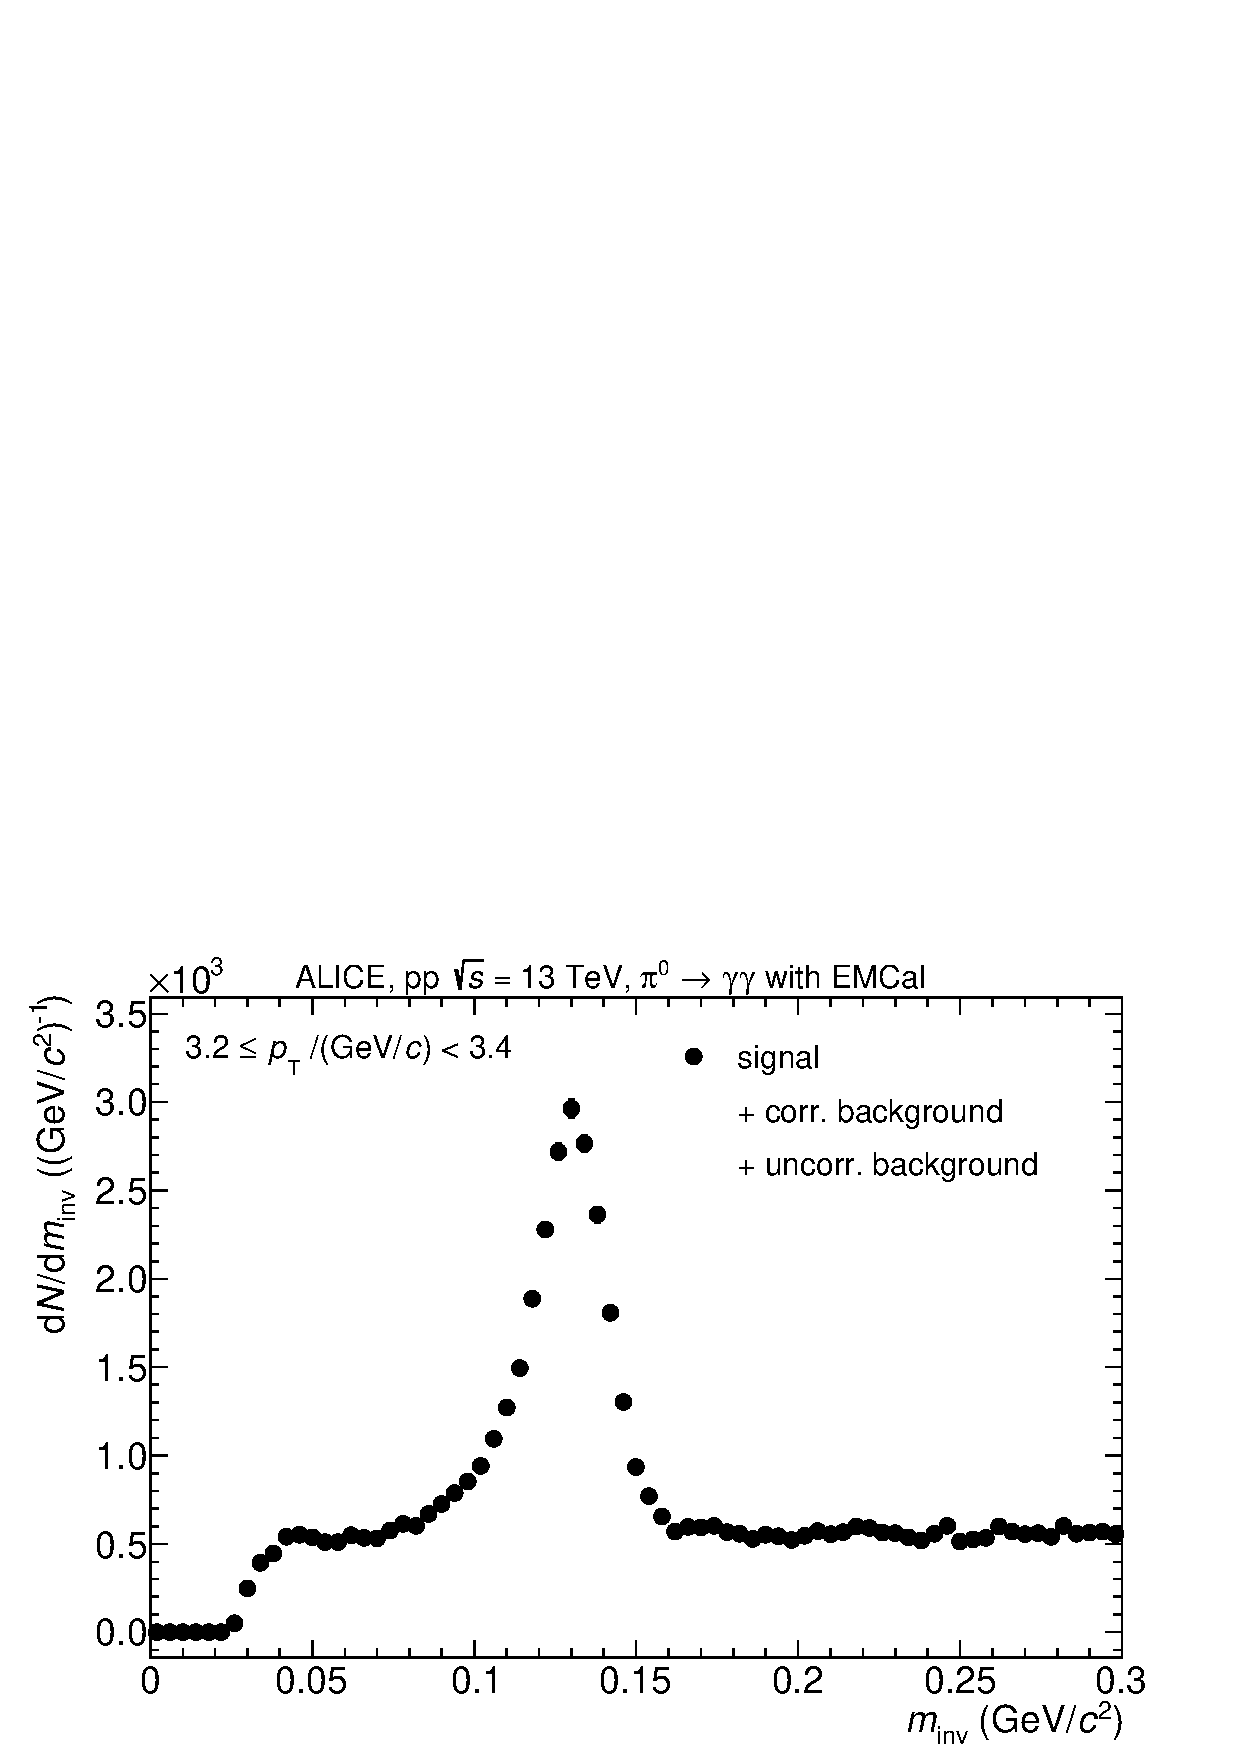
\includegraphics[width=.75\linewidth]{hSignalPlusBkg.pdf}
\caption{Projektion von Abbildung \ref{figInvMassPt_a} im $p_{\text{T}}$-Intervall $(3,2 - 3,4) (\text{GeV/}c)$. Es ist ein deutlicher Peak um $m_{\pi^{0}} \approx 0\,135\text{ GeV/}c^{2}$ zu erkennen, aber auch Untergrund, da das Signal zu höheren Massen gaußförmig abklingen sollte. Bei $m_{\text{inv}} < m_{\pi^{0}}$ kann Signal vorliegen, das aus konvertierten Photonen besteht, weshalb eine Aussage über die Form, beziehungsweise den Untergrund dort schwer möglich ist.}
\label{figSignalPlusBkg}
\end{figure}
\newline
Abbildung \ref{figSignalPlusBkg} zeigt die Anzahl der \textit{Clusterpaare} in Abhängigkeit der invariante Massen im $p_{\text{T}}$-Intervall von $(3\,2 - 3\,4)(\text{GeV}/c)$.
Die in Abbildung \ref{figInvMassPt_a} beschriebene Anhäufung der Datenpunkten zeigt sich auch hier deutlich und wird im Folgenden als Peak bezeichnet.
Der Peak besteht wie zuvor erwähnt hauptsächlich aus Signal.
\newline
Im folgenden Abschnitt wird eine Methode zur Abschätzung des unkorrelierten Untergrunds vorgestellt. 